\documentclass[float=false]{standalone}

\usepackage{tikz}
\usetikzlibrary{calc,shapes,chains,scopes,shapes.multipart}

\begin{document}

\def\task{\nodepart{one}}
\def\time{\nodepart{two}}

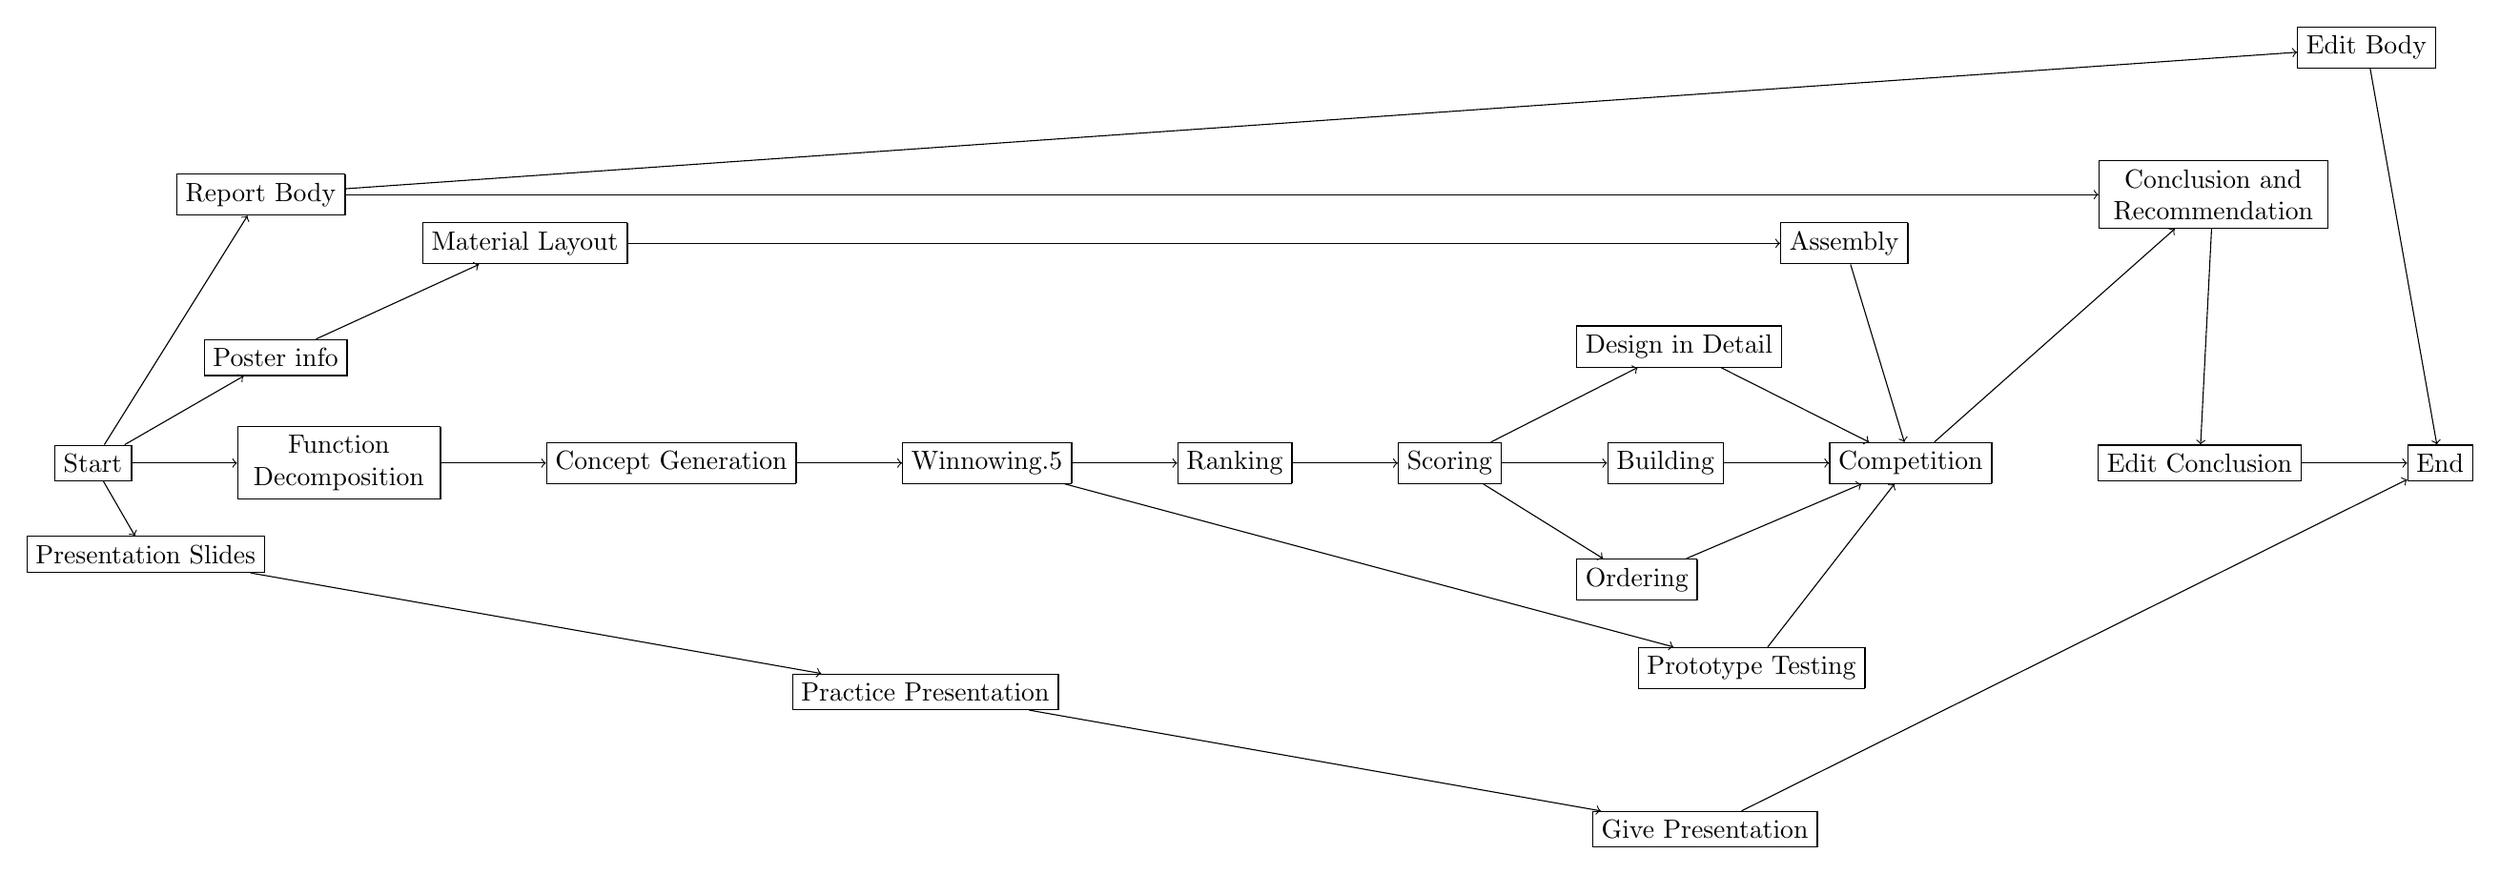
\begin{tikzpicture}[
	node distance=4em,
	every on chain/.style={
		join,
		rectangle split,
		rectangle split horizontal,
		rectangle split parts=2,
		rectangle split ignore empty parts,
		align=center,
		draw,
	},
	every join/.style={->},
]
{
	[start chain=main]
	\node (start) [on chain] {Start};
	{ [start branch=report]
		\node (reportbody) [on chain=going {at=(\tikzchainprevious),shift=(58:6em)}] {Report Body\time7};
		{ [start branch=editbody]
			\node (editbody) [on chain=going {at=(\tikzchainprevious),shift=(4:40em)}] {Edit Body\time4};
		}
	}
	{ [start branch=poster]
		\node (posterinfo) [on chain=going {at=(\tikzchainprevious),shift=(30:4em)}] {Poster info\time3};
		\node (materiallayout) [on chain=going above right] {Material Layout\time1};
		\node (assembly) [on chain=going {at=(\tikzchainprevious),shift=(0:25em)}] {Assembly\time1};
	}
	{ [start branch=presentation]
		\node [on chain=going {at=(\tikzchainprevious),shift=(-60:2em)}] {Presentation Slides\time5};
		\node [on chain=going {at=(\tikzchainprevious),shift=(-10:15em)}] {Practice Presentation\time2};
		\node [on chain=going {at=(\tikzchainprevious),shift=(-10:15em)}] {Give Presentation\time1};
	}
	\node (functiondecomp) [on chain] {\nodepart[text width=7em]{one}Function Decomposition\time1};
	\node (conceptgeneration) [on chain] {Concept Generation\time2};
	\node (winnowing) [on chain] {Winnowing\time0.5};
	{ [start branch=prototype]
		\node (prototypetesting) [on chain=going {at=(\tikzchainprevious), shift=(-15:15em)}] {Prototype Testing\time3};
	}
	\node [on chain] {Ranking\time1};
	\node (scoring) [on chain] {Scoring\time2};
	{ [start branch=design]
		\node [on chain=going above right] {Design in Detail\time9};
	}
	{ [start branch=ordering]
		\node [on chain=going below right] {Ordering\time6};
	}
	\node (building) [on chain] {Building\time10};
	\node (competition) [
		on chain,
		join=with main/design-end,
		join=with main/ordering-end,
		join=with main/poster-end,
		join=with main/prototype-end,
	] {Competition\time1};
	{ [continue branch=report]
		\node (conclusion) [on chain=going {at=(\tikzchainprevious), shift=(0:37em)},join=with competition] {\nodepart[text width=8em]{one} Conclusion and Recommendation\time2};
		%\node (editconclusion) [on chain=going {at=(\tikzchainprevious),shift=(-55:1.5)}] {Edit Conclusion\time2};
		\node (editconclusion) [on chain, right=of competition] {Edit Conclusion\time2};
		\node (end) [
			on chain,
			join=with main/presentation-end,
			join=with main/report/editbody-end,
		] {End};
	}
}
\end{tikzpicture}

\end{document}

